\chapter{Results}
\label{sec:results}
This chapter discusses how I took the results of my survey and began to look at the different ways that applications use local IPC, as well as my work testing the security of this communication.

\section{General Results}
\label{sec:generalResults}
Based on the results of the survey that I received, I am able to make some general statements about the way that the three types of local IPC that I am studying---named pipes, Internet sockets that use the loopback interface, and UNIX domain sockets---are used by applications.  All of this data is reflected in Table~\ref{appendix:allData}.  I received twenty-two responses from the over 250 people that my survey was sent out to, roughly a 9\% response rate.  I was hoping to have more data, but was able to find results, even with the limited responses.

I collected data on the number of anonymous pipes that an application had open to be able to compare to the local IPC methods I studied.  Anonymous pipes were used the most, with many applications having tens, or even hundreds of them open at a time.  While these are used the most, I consider them to be a secure form of local IPC since, similar to \texttt{socketpair} sockets, the process creating one must explicitly give another process access.

The most notable result when looking through my data is how rarely named pipes are used by applications.  Only three applications used named pipes at all, and all three were applications created by Adobe.  In the Man-in-the-Machine paper that prompted my thesis~\cite{MitMa}, named pipes were one of the two most-common ways that the authors exploited local IPC.  However, all of their named pipe exploits occurred only on Windows.  This could imply that they also found few Mac applications that used named pipes or that applications running on Mac and Linux operating systems use UNIX domain sockets instead of named pipes.  Because of the low number of applications that utilized named pipes, I did not study their security, so the rest of this chapter will exclusively be about Internet sockets and UNIX domain sockets.

Internet sockets using TCP and UDP and connecting over the loopback interface were less commonly used that anonymous pipes.  Only three applications had at least ten TCP or UDP sockets open and listening on the loopback interface at any time.  However, one of those, mDNSResponder, averaged over sixty listening UDP sockets at a time.  Other than this outlier, there was little difference between the number of TCP or UDP sockets open at a time.  This could be due to the low chance that a UDP packet, even though it does not have guaranteed delivery, is dropped in transit, so many applications that may use TCP for networked communication opt for the lower overhead of UDP for local communication.

Finally, UNIX domain sockets are used on average more than named pipes or Internet sockets.  Twenty-one applications had at least ten UNIX sockets open at a time, with seven of these having at least thirty-five open on average.  These statistics do not differentiate between named and unnamed \texttt{socketpair} UNIX sockets, but from examining the detailed output of my survey, it looks like most UNIX domain sockets are created by the \texttt{socketpair} system call.

\section{Applications}
\label{sec:applications}
I decided to look at four different applications: Spotify, Microsoft Visual Studio Code (VS Code), launchd, and mDNSResponder.  I chose Spotify because it was running on over 50\% of of machines in my survey and it uses a diverse set of local IPC resources including local TCP and UDP Internet sockets and UNIX domain sockets.  VS Code was running on relatively few machines, but has many named UNIX domain sockets which I could both fuzz and attempt server impersonation.  launchd also had many named UNIX domain sockets and, since it boots the computer, is responsible for many system-wide functions that must be kept secure.  Finally, mDNSResponder has a huge number of listening UDP sockets and named UNIX domain socket endpoints which gave me many opportunities to find results.

These four applications gave me broad coverage of many factors that I wanted to look into.  Spotify and VS Code are user programs that use multiple processes that work together.  On the other hand, launchd is a single process that is the first process created at boot time, giving it the process ID of 1.  It is also owned by root, not a normal user.  mDNSResponder is another single process but is owned by the \_mdnsresponder user.

\begin{table}
\centering
\begin{scriptsize}
\begin{tabular}{ l | l | l | l | l | l}
APP NAME & NUM MACHINES & FIFOS & LOCAL TCP(TOTAL) & LOCAL UDP(TOTAL) & UNIX Sockets \\ \hline
Spotify & 12 & 0 & 1(9) & 3(3) & 10 \\ \hline
VS Code & 2 & 0 & 2(10) & 0(0) & 22 \\ \hline
launchd & 22 & 0 & 4(4) & 2(2) & 36 \\ \hline
mDNSResponder & 22 & 0 & 1(3) & 62(62) & 44 \\ \hline
\end{tabular}
\caption{Average Local IPC Resources for Each Application}
\label{tab:applicationData}
\end{scriptsize}
\end{table} 

These applications also use different forms of local IPC.  Table~\ref{tab:applicationData} shows the distribution of local IPC resources for each.  As stated above, very few applications on OS X use named pipes, so I did not study how applications used FIFOs since they were so rare.  Spotify was being run on over 50\% of surveyed machines, and on average, it had one TCP port and three UDP ports listening on the localhost address.  It also averaged ten UNIX domain sockets open at any time.  VS Code was run on relatively few machines, just under 10\%, but had two listeing TCP sockets and fourteen UNIX domain sockets, many of them named in the filesystem.  launchd and mDNSResponder were both running on 100\% of computers.  launchd had four local TCP sockets listening, two UDP sockets, and thirty-six UNIX domain sockets open on average.  mDNSResponder had one local TCP socket, sixty-two local UDP sockets, and forty-four UNIX domain sockets.  launchd and mDNSResponder also both had named UNIX sockets, not only \texttt{socketpair} sockets.

These applications also use local inter-process communication between processes owned by different users.  For example, Spotify has UNIX domain socket connections between its processes, which are owned by a normal user.  However, it also has sockets where the user at the other end is root or \_mdnsresponder.  These differences in endpoint privileges could be the basis for privilege escalation or execution hijacking as root user, and therefore are especially worth studying because of the increased risk.

Next, I will go into more depth on each application, describing its local IPC footprint as well as detailing the steps I took while investigating its security.  This will include fuzzing TCP and UDP endpoints through the loopback interface and UNIX domain sockets.

\section{Spotify}
\label{sec:spotify}
Spotify has a broad local IPC footprint.  Each instance of the Spotify application runs two different processes, Spotify and Spotify Helper.  Additionally, a third type of process also is used occasionally, SpotifyWebHelper, but this was only seen on two machines in the survey and I was unable to reproduce it while testing.  When I was testing the Spotify application, it had two TCP sockets listening on any address on ports 57621 and 57819.  It also had three UDP sockets listening on ports 1900, 62152 and 57621.  Finally, it had eleven open UNIX domain socket endpoints.  We will dive into each of these categories deeper.

\subsection{Spotify UDP}
\label{sec:spotifyUdp}
Spotify has three UDP ports listening on any IP address when it runs.  One is always listening on port 1900 and another is on a random port.  Unfortunately, I was unable to find any communication over these ports.

However, the last UDP port is listening on port 57621.  This port sends a regular message every thirty seconds.  I believe that this is a ``heartbeat'' message sent to the local broadcast address for both the loopback interface and the Wifi radio interface of my computer.  This message could be used as a way to find other instances of Spotify running nearby, or as a way for some software to see that this instance of Spotify is still running.  The data of each message is always exactly forty-four bytes long, with the first eight bytes reading \texttt{SpotUdp0}.  While the data is different for each instance of Spotify that I run, within an instance, the data is always the same, meaning once I start Spotify, the data sent every thirty seconds will always be exactly the same.  Since I have many examples of these messages, I was able to effectively fuzz this endpoint.

I created a Python program that would send the two pieces of the data section to \textit{radamsa} and use the result to build a new message.  I then sent this new, random message to UDP port 57621 via localhost.  I did this over 500,000 times.  After each message, I checked to see whether Spotify was still running.  None of these random strings caused a crash in Spotify.

Even though I was unable to find any messages to the other two UDP ports, I still fuzzed them using the same messages that I fuzzed port 57621 with.  I fuzzed both of these ports over 500,000 times as well and never crashed Spotify.  I then moved on to the TCP sockets to see if I would be able to find a bug while fuzzing these.

\subsection{Spotify TCP}
\label{sec:spotifyTcp}
When the Spotify application runs, it establishes many TCP connections across the Internet to get the music and other data for the user.  However, there are also two sockets that listen on any interface; one is always on port 57621 while the other is random.  Using Wireshark, I could not find any messages being sent on either of these ports for any instance of Spotify.

Again, like the last two UDP ports, I still fuzzed these endpoints, even without finding any messages being sent to these ports.  When I fuzzed TCP port 57621 using the UDP heartbeat message, I was unable to cause a crash in Spotify.  However, when I fuzzed the random TCP port, something else happened.  Each time I created a connection, the socket would immediately be closed for me to write.  When I investigated further, whenever I connected to this socket, I immediately received a message stating that the type is Tier1 and the version is 1.0, as shown in Figure~\ref{fig:spotifyTcpResponse}.  Then, the socket would be closed, all before I would be able to send a message.  I am not sure what this message means, but it could be a way for other Spotify processes or applications that interact with Spotify to get version information.  Unfortunately, since the socket was being closed immediately, I was unable to fuzz it.

\begin{figure}
\centering
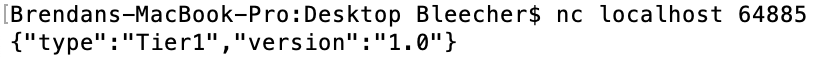
\includegraphics[width=1\textwidth]{spotifyMessage.png}
\caption{Message Received from Spotify TCP Port}
\label{fig:spotifyTcpResponse}
\end{figure}

\subsection{Spotify UNIX Domain Sockets}
\label{sec:spotifyUnix}
Finally, I investigated the UNIX domain sockets that Spotify opened.  For each instance of Spotify created during testing, the Spotify application would have eleven UNIX domain socket endpoints open.  These were split among one instance of the Spotify process and two instances of the Spotify Helper process.  Of these eleven endpoints, eight were created using \texttt{socketpair} and shared between the various Spotify processes.  There was one pair within the Spotify process, and another pair between each Spotify Helper process and the Spotify process.  Finally, there was a pair between the two Spotify Helper processes.  Since no other process was given any of these endpoints, there was no way to send any messages or attempt to fuzz these endpoints.  However, there were also three UNIX domain sockets that were connected to named UNIX sockets.  One was connected to a socket owned by both launchd and syslogd.  The security of this communication will be discussed in Section~\ref{sec:launchdUnix}.  The other two were both connected to a socket owned by mDNSResponder.  This will be examined in Section~\ref{sec:mdnsUnix}.

\begin{table}
\centering
\begin{scriptsize}
\begin{tabular}{ l | l | l | l }
\textbf{Form of Local IPC} & \textbf{Socket Type} & \textbf{Attack Vector} & \textbf{Result} \\ \hline
Internet Domain Socket & 1 TCP Socket & Input-based & Fuzzed with no crash \\ \hline
Internet Domain Socket & 3 UDP Sockets & Input-based & Fuzzed with no crash \\ \hline
UNIX Domain Socket & 3 named connections & Input-based & Owned by others, could not fuzz \\ \hline
UNIX Domain Socket & 8 \texttt{socketpair} endpoints & Input-based & Cannot fuzz \\ \hline
\end{tabular}
\caption{Summary of my Investigation into Spotify}
\label{tab:spotifyData}
\end{scriptsize}
\end{table} 

\subsection{Spotify Conclusion}
\label{sec:spotifyConclusion}
Based on my research into Spotify, summarized in Table~\ref{tab:spotifyData}, I believe that this application is fairly secure against local input-based vulnerabilities.  I was unable to crash Spotify using any of the open UDP or TCP sockets.  Additionally, its use of UNIX domain sockets is very secure since almost all of them are created using \texttt{socketpair} and therefore cannot be directly given input by an outside process.

\section{VS Code}
\label{sec:code}
VS Code only uses two of the forms of local IPC that I studied: local TCP connections and UNIX domain sockets.  However, the biggest reason that I chose to look at VS Code is because it has so many named UNIX sockets.  Additionally, some of these sockets have the same name for each instance of VS Code while others have random suffixes each time.  This gives an interesting contrast to study.  VS Code is made up of the processes Code Helper and Electron.  There is always only one running process of Electron, but depending on the number of windows and tabs open, there may be many running instances of Code Helper.

\subsection{VS Code TCP}
\label{sec:codeTcp}
VS Code averaged two listening TCP ports, according to my survey data.  The ports chosen were always random, so I needed to find the port each time I started a fuzzing session.  When I originally fuzzed these ports with random data, I was always returned the message ``WebSockets request was expected.''  After doing research, I found that this meant that it was looking for an HTTP request.  Therefore, I created an HTTP GET request to get the repository holding the research for this thesis from GitHub and used this as my genuine communication example.

When I used this message to fuzz the VS Code endpoint, the program would end between fifty and one hundred messages into fuzzing because the port had been closed.  Whenever I went back to my open instance of VS Code, my VIM extension no longer worked.  VS Code was no longer using VIM keybindings nor was it using the normal keyboard keys and shortcuts.  This experiment was repeated three times, and each time the VIM extension crashed.  I had crashed this extension.  This finding represents a bug in the way that VS Code parses input to its random TCP ports since it does not correctly handle the input I was sending.  This bug could also constitute a vulnerability, which, if exploitable, could allow an attacker to either hijack execution or disclose personal information.  Therefore, this is a significant finding.

\subsection{VS Code UNIX Domain Sockets}
\label{sec:codeUnix}
In addition to its TCP sockets, VS Code also has many UNIX domain sockets,  four of which are named.  One is named based on the version number and the word `main', hereafter known as the main socket.  One is named off of the version number and the word `shared', known as the shared socket.  The last two are named using either the word `git' or `ipc' and followed by a random suffix; I call these the git and ipc sockets, respectively.  These random socket names were likely created with the \texttt{mktemp} library call or utility to create a name that is guaranteed to be unique in the filesystem.

When fuzzing the main socket, I used a six-byte message as my seed that was sent when the application was being closed.  However, after fuzzing over 500,000 times with variations of this message, VS Code did not crash or function incorrectly.

However, since the name of the main socket does not change, I deleted the socket from the filesystem and created it again myself.  Then, I tried to open VS Code.  I received a message saying that another instance of VS Code was running.  I had created a Denial-of-Service attack by opening the main socket myself.  VS Code must have checked the return value of the bind call, seen that this name in the filesystem was already taken, and decided that an instance was already running.  Since I had created this socket, no other version of VS Code would be able to run without first deleting the socket from the file system and killing any process that had it open or restarting the entire machine.

The next socket that I looked at was the shared socket.  By impersonating this socket, I found a forty-five byte message that was sent from a client when VS Code started.  Using this message to fuzz the shared socket, I was unable to cause a crash after 500,000 iterations.

I then investigated the git socket.  Since it has a random suffix, I could not create this socket before I had a running instance of VS Code.  However, I did delete the socket and recreate it myself, but did not find any sample messages.  When I attempted to fuzz this socket, I received a BrokenPipeError in Python after two messages were successfully sent.  A BrokenPipeError in Python means that the remote communication endpoint has closed the socket for reading, but the local endpoint is still sending data.  I hypothesize, since this error always occurred after two successful sends, that this could be a security measure put in place by VS Code.  This socket may never expect to see more than two messages from the same client, so if it ever sees a third message, it closes that connection for reading because it believes something nefarious is happening.  It is also possible that this could be an error in the way that the socket is being used, but since it always occurred after exactly two successful messages, I believe that it is for security purposes.

The last named socket is the ipc socket.  Again, this socket has a random suffix so I cannot create it before I started VS Code.  Once I started VS Code, I would see in the output of \texttt{lsof} that this socket was open and connected to another UNIX domain socket owned by another instance of the Code Helper process.  However, when I tried to delete this socket from the file system to create my own version, I found that this socket did not exist.  If I tried to connect to the ipc socket as a client, I would receive an error stating that the file did not exist.

This means that VS Code created this socket and created the connections it needed while the application was starting, then immediately called \texttt{unlink} on the socket.  This would remove the link count of the socket, decrementing it to zero.  Since the link count was zero, it would no longer show up in the filesystem, which explains my findings.  However, since this socket was still being used, it would not actually be garbage collected by the system until all processes referencing the file exited.  Therefore, the two separate Code Helper processes were able to connect and still communicate while being sure that no other process could snoop on the communication.

I do not know why VS Code uses this system for the ipc socket, especially when it has so many \texttt{socketpair} sockets open at the same time, even between the two processes connected by the ipc socket.  However, the usage of the ipc socket is, in practice, the same as a \texttt{socketpair} socket since no other process can join the conversation.

\begin{table}
\centering
\begin{scriptsize}
\begin{tabular}{ l | l | l | l }
\textbf{Form of Local IPC} & \textbf{Socket Type} & \textbf{Attack Vector} & \textbf{Result} \\ \hline
Internet Domain Socket & 2 TCP Sockets & Input-based & Fuzzing caused VIM extension to crash \\ \hline
UNIX Domain Socket & Named ``main'' socket & Input-based & Fuzzed with no crash \\ \hline
UNIX Domain Socket & Named ``main'' socket & Server impersonation & Denial-of-Service Attack \\ \hline
UNIX Domain Socket & Named ``git'' socket & Input-based & Possible security feature \\ \hline
UNIX Domain Socket & Named ``ipc'' socket & Input-based & Cannot fuzz \\ \hline
UNIX Domain Socket & Named ``shared'' socket & Input-based & Fuzzed with no crash \\ \hline
UNIX Domain Socket & 18 \texttt{socketpair} endpoints & Input-based & Cannot fuzz \\ \hline
\end{tabular}
\caption{Summary of my Investigation into VS Code}
\label{tab:codeData}
\end{scriptsize}
\end{table} 

\subsection{VS Code Conclusion}
\label{sec:codeConclusion}
My research, outlined in Table~\ref{tab:codeData}, has shown that VS Code is not immune to input-based vulnerabilities over local IPC.  Through my fuzzing, I crashed a VIM extension that was open in VS Code.  Additionally, I caused a Denial-of-Service attack by opening the main UNIX socket before opening the VS Code application.  While VS Code does use some security features, like closing the connection if the git socket receives more than two messages and immediately \texttt{unlink}ing the ipc socket, it still is vulnerable and must be fixed, lest it be exploited.

\section{launchd}
\label{sec:launchd}
I chose to text launchd because it is the process that helps boot the machine, as well as starting many services, or daemons.  It is responsible for creating and maintaining many necessary services, such as networking, logging and showing images on the screen.  launchd uses local TCP and UDP sockets, as well as many named UNIX domain sockets.

\subsection{launchd TCP}
\label{sec:launchdTcp}
My survey results showed that launchd averaged four open TCP sockets at a time.  However, no matter when I tried to find these sockets on my own computer, I was unable to find an open TCP socket that launchd was listening to.  Therefore, since I could not recreate this result, I was unable to fuzz any TCP sockets for launchd.

\subsection{launchd UDP}
\label{sec:launchdUdp}
launchd averaged two open UDP sockets, one listening on port 137 and the other on port 138, both listening on any interface.  These ports are the netbios-ns and netbios-dgm ports.  NetBIOS was a way for computers to communicate on a local network.  The netbios-ns port was used to get the NetBIOS name of another computer on the network and netbios-dgm was used to send datagrams within the network.  I used \textit{Wireshark} to find sample messages being sent to these ports, and found two examples of mDNS responses.  To fuzz these sockets, my program randomly chooses one message, sends it to \textit{radamsa} to modify and then randomly chooses a port to send it to.  In this way, both messages were randomly being sent to both ports, maximizing the possiblity of a crash.  Even with this process, fuzzing both of these ports did not cause launchd to crash.

\subsection{launchd UNIX Domain Sockets}
\label{sec:launchdUnix}
Unlike every other process that I looked at, a majority of launchd's UNIX domain sockets were not \texttt{socketpair} sockets.  In face, launchd had no \texttt{socketpair} endpoints; it only had named UNIX domain sockets.  While the survey results show that launchd had on average thirty-six open UNIX domain sockets, each socket was opened twice, so there were only eighteen different sockets open.  I attempted to fuzz six of these, representing one-third of the open sockets.  I was unable to find sample messages for any of these UNIX domain sockets, so I used the same sample messages from fuzzing the launchd UDP sockets as the seeds for my UNIX domain socket messages.

Every running application that does logging connects to a named socket owned by launchd; this was the first socket that I fuzzed.  Spotify, VS Code and mDNSResponder all had a connection to this socket.  This socket was a datagram UNIX socket, and the only one that I found in my research.  I fuzzed this socket over 500,000 times and was not able to crash launchd.  I had the same result with two stream sockets that worked with remote procedure calls and a VPN.

The other three UNIX sockets that I attempted to fuzz were part of the system keychain, a port-mapping software, and the software that multiplexes access to the USB port.  While fuzzing these sockets, a BrokenPipeError would be thrown often, and quite regularly.  The system keychain socket would throw the error after one or two messages was sent successfully, then to every message for a short time period after.  Similarly, when fuzzing the port-mapping socket, the error would occur after about forty messages, and then to every message from every connection for a short time.  This seems to show that the process owning the socket sees that too many messages are being sent, and could be malicious.  It then closes the socket for reading for a short amount of time to hopefully discourage the malicious user from continuing.

The USB socket also would throw a BrokenPipeError after the first message it received from every single connection.  Like with the git UNIX domain socket from VS Code in Section~\ref{sec:codeUnix}, this could be a security feature.  Also like VS Code, it is difficult to tell the exact motivation behind this function, or even if it is intended.  However, based on my research, it is plausible that this error is meant to decrease the likelihood of an input-based attack.

\begin{table}
\centering
\begin{scriptsize}
\begin{tabular}{ l | l | l | l }
\textbf{Form of Local IPC} & \textbf{Socket Type} & \textbf{Attack Vector} & \textbf{Result} \\ \hline
Internet Domain Socket & 4 TCP Sockets & Input-based & Could not reproduce \\ \hline
Internet Domain Socket & 2 UDP Sockets & Input-based & Fuzzed with no crash \\ \hline
UNIX Domain Socket & 3 named sockets & Input-based & Fuzzed with no crash \\ \hline
UNIX Domain Socket & 3 named sockets & Input-based & Possible security feature \\ \hline
\end{tabular}
\caption{Summary of my Investigation into launchd}
\label{tab:launchdData}
\end{scriptsize}
\end{table} 

\subsection{launchd Conclusion}
\label{sec:launchdConclusion}
From my research, shown in Table~\ref{tab:launchdData}, launchd seems to be secure against many local IPC-based input attacks.  I could not recreate its TCP sockets and fuzzing its UDP sockets never caused a crash.  While it has many named UNIX domain sockets, it appears that many of these implement some sort of security plan to diminish the possibility of input-based attacks.  The sockets that do not seem to have this plan did not cause a crash of launchd while being fuzzed, so they are secure as far as I have tested.

\section{mDNSResponder}
\label{sec:mdns}
The final process that I tested is mDNSResponder, which is responsible for different parts of networking, including DNS, AirDrop, and finding nearby printers.  mDNSResponder had the largest local IPC footprint of the four applications that I studied, averaging sixty-two listening UDP sockets and forty-four UNIX domain sockets.  This set up a large testing ground for my research.

\subsection{mDNSResponder TCP}
\label{sec:mdnsTcp}
According to my survey, mDNSResponder had, on average, one TCP socket listening on any interface.  However, this socket was always in the `CLOSED' state, which means that it has not started to listen yet, or had a connection and closed it and is not yet listening for any more.  Therefore, since this socket was not listening for incoming connections, I could not fuzz the single, local mDNSResponder TCP socket.

\subsection{mDNSResponder UDP}
\label{sec:mdnsUdp}
mDNSResponder always has two sockets listening on the mdns port, port number 5353.  This can be done by setting the SO\_REUSEPORT on all of the sockets before binding, and can help load-balance across multiple sockets.  I found two sample messages send to port 5353 by using \textit{Wireshark}, and used these as my seed messages for fuzzing.  Each iteration, one of the two messages was randomly selected and then randomly modified, then sent to the port.  I was unable to cause a crash of mDNSResponder or a slowdown in Internet speed from this fuzzing.

\subsection{mDNSResponder UNIX Domain Sockets}
\label{sec:mdnsUnix}
As mentioned above, mDNSResponder has over forty UNIX domain sockets open at any one time.  There are four endpoints open within the process, representing four of the total UNIX socket endpoints.  The other forty are all connected to the same named UNIX domain socket.  I fuzzed this named socket using a thirty-two-byte message that I received when I created my own version of this socket.  Even after 500,000 iterations, Internet traffic was no slower and mDNSResponder had not crashed.

However, when I created my own instance of the named UNIX socket after deleting the real version, most Internet traffic from my computer failed.  All webpages failed to load, and I could no longer get music from Spotify.  This was essentially a Denial-of-Service attack, where I denied access to most of the rest of the Internet.  The only way to bring back Internet access was to restart the entire machine and let mDNSResponder create the real socket again.

\begin{table}
\centering
\begin{scriptsize}
\begin{tabular}{ l | l | l | l }
\textbf{Form of Local IPC} & \textbf{Socket Type} & \textbf{Attack Vector} & \textbf{Result} \\ \hline
Internet Domain Socket & 1 TCP Socket & Input-based & Always CLOSED \\ \hline
Internet Domain Socket & 62 UDP Sockets & Input-based & Fuzzed with no crash \\ \hline
UNIX Domain Socket & 1 named socket & Input-based & Fuzzed with no crash \\ \hline
UNIX Domain Socket & 1 named socket & Server impersonation & Denial-of-Service Attack \\ \hline
UNIX Domain Socket & 4 \texttt{socketpair} endpoints & Input-based & Cannot fuzz \\ \hline
\end{tabular}
\caption{Summary of my Investigation into mDNSResponder}
\label{tab:mdnsData}
\end{scriptsize}
\end{table} 

\subsection{mDNSResponder Conclusion}
\label{sec:mdnsConclusion}
Based on all of my research, condensed into Table~\ref{tab:mdnsData}, it seems that mDNSResponder is secure against local input-based vulnerabilities.  However, if its named UNIX domain socket is deleted, the machine loses most access to the rest of the outside world.  While this attack is not an input-based attack, it uses local IPC channels as the attack vector to stop Internet access.
